\chapter{Анализ результатов тестирования и оптимизация генерируемого кода}

В данном разделе проводится анализ результатов запусков тестов производительности на виртуальных машинах V8 и SpiderMonkey. 
Кроме того, предлагаются способы оптимизации обнаруженных <<узких>> мест и описываются реализации некоторых из предложенных оптимизаций. 

\section{Методика тестирования}

Запуск тестов производил на компьютере со следующими характеристиками:
\begin{itemize}
\item Процессор: Intel Core 2 6400 с частотой 2.13 GHz.
\item Размер оперативной памяти: 4 Gb.
\item Операционная система: Ubuntu 12.10 64-bit.
\end{itemize}

Для запуска JavaScript кода, в том числе сгенерированного компиляторами Kotlin и Dart2js, использовались виртуальные машины V8 версии 3.17 и SpiderMonkey 17 версии (mozjs17). Запуск тестов с использованием V8 никакие ключи не использовались. А при запуске тестов в SpiderMonkey использовался следующий набор ключей: <<\path$--methodjit$ \path$--typeinfer$>>. Первый параметр включает JIT компиляцию методов, второй -- включает сбор информации о типах переменных и дальнейшее использования этой информации для оптимизаций.
Для запуска тестов на языке Dart использовалась виртуальная машина DartVM. Виртуальная машина языка Dart и компилятор Dart2js были взяты из Dart SDK версии 0.4.2.8.

Каждое измерение состоит из двух основных этапов, каждый длительностью две секунды. Длительность этапов была подобрана так чтобы этого времени хватало на стабилизацию процессов внутри виртуальной машины. Первый запуск нужен для того что бы дождаться пока виртуальная машина перейдет в стабильное состояние. Так же, на этом этапе осуществляется так называемый <<прогрев>> виртуальной машины. Данная процедура, позволяет виртуальной машине собрать необходимую информацию о коде, чтобы провести оптимизации и выполнять тест максимально быстро на втором этапе.
Во время основного запуска измеряется количество итераций, запущенных в течении двух секунд, и то сколько реально времени на это было потрачено. 
В конце каждой итерации выполняется проверка результатов и в случае если они не соответствуют эталонному значению тестирование экстренно завершается. Результатом работы теста является среднее время выполнения одной итерации во время основного запуска.

\section{Richards}

Результаты, полученные на начальном этапе, когда еще не были сделаны никакие оптимизации, на тест Richards представленны на рисунке \ref{richards_0}. Столбец <<Фактор>> показывает во сколько раз время полученное на данном тесте больше времени теста на Dart.

% \begin{table}[h]
% \centering
% \caption{This table shows some data}
% \end{table}

\begin{figure}[ht!]
% \centering
\begin{minipage}[t]{\linewidth}
\includegraphics[width=0.65\textwidth]{images/richards_0.png}
\end{minipage}
~
\put(-170,175){\begin{minipage}[h]{\linewidth}
\begin{tabular}{|l|c|c|}
    \hline
    ~                    & Время (мкс) & Фактор \\ \hline
    Dart                 & 2721.09     & 1.0    \\ \hline
    Dart2JS(v8)          & 5101.78     & 1.87   \\ \hline
    JavaScript (v8)      & 3683.24     & 1.35   \\ \hline
    Kotlin2JS (v8)       & 19900.99    & 7.31   \\ \hline
    Dart2JS(mozjs17)     & 48571.43    & 17.85  \\ \hline
    JavaScript (mozjs17) & 6876.28     & 2.53   \\ \hline
    Kotlin2JS (mozjs17)  & 111722.22   & 41.06  \\ \hline
\end{tabular}
\end{minipage}}
\caption{Результаты теста Richards без оптимизаций}
\label{richards_0}
\end{figure}

Из данной диаграммы видно, что при запуске на виртуальной машине V8 тест, скомпилированный с помощью компилятора Kotlin, уступает тесту, скомпилированному с помощью Dart2js, примерно в 4 раза, а тесту написанному на JavaScript -- более чем в 5 раз. При запуске на mozjs17 эта разница, при сравнении с тестом написанным на JavaScript увеличивается до примерно 15 раз и в случае с Dart2js уменьшается до 2 раза. Безусловным лидером данного и всех остальных тестов является код написанный на Dart и запущенный в DartVM.

Если открыть код, получившейся в результате компиляции с помощью компилятора Kotlin, не трудно заметить, что все обращения даже внутри пакета осуществляются по полному имени (см. листинг \ref{example_with_package}). Такого рода обращений в получившемся коде очень много и в случае большой вложенности пакетов это может отрицательно сказаться на производительности. 

\begin{code}
\begin{JavaScript}[caption=Пример код с обращением по полному имени внутри того же пакета, label=example_with_package]
...
_ = {
org: Kotlin.definePackage({
  jetbrains: Kotlin.definePackage({
    kotlin: Kotlin.definePackage({
      benchmarks: Kotlin.definePackage({
        Richards_from_darts: Kotlin.definePackage({
          js: Kotlin.definePackage({
            //...
            addIdleTask: function (id, priority, queue, count) {
            this.addRunningTask(id, priority, queue, new _.org.jetbrains.kotlin.benchmarks.Richards.js.IdleTask(this, 1, count));
            }
            //...
\end{JavaScript}
\end{code}

Экспериментально было подтвержденно, что для виртуальной машины V8 это действительно так -- этот же тест, но с меньшей вложенностью пакетов выполняется примерно на 30\% быстрее. А для виртуальной машины mozjs17 такое изменение никакого влияния на производительность не оказало (см. рисунок \ref{richards_i}).

\begin{figure}[ht!]
% \centering
	\begin{subfigure}[b]{0.65\textwidth}
	% \centering
  \begin{minipage}[t]{\linewidth}
	\includegraphics[width=\textwidth]{images/richards_i_v8.png}
  \end{minipage}
  ~
  \put(-10,217){\begin{minipage}[h]{\linewidth}
  \begin{tabular}{|l|c|}
      \hline
      ~                    & Время (мкс) \\ \hline
      Kotlin2JS(без изм.)  & 19900.99    \\ \hline
      +Без пакетов(package)& 14262.41    \\ \hline
      +Closure-compiler    & 8721.09     \\ \hline
      +Inline accessors    & 5859.64     \\ \hline
  \end{tabular}
  \end{minipage}}

	\caption{Результаты измерений на V8}
  \end{subfigure}

  \begin{subfigure}[b]{0.65\textwidth}
	% \centering
  \begin{minipage}[t]{\linewidth}
	\includegraphics[width=\textwidth]{images/richards_i_mozjs17.png}
  \end{minipage}
  ~
  \put(-10,217){\begin{minipage}[h]{\linewidth}
  \begin{tabular}{|l|c|c|}
      \hline
      ~                    & Время (мкс) \\ \hline
      Kotlin2JS(без изм.)  & 111722.22   \\ \hline
      +Без пакетов(package)& 113833.33   \\ \hline
      +Closure-compiler    & 63000.09    \\ \hline
      +Inline accessors    & 25125       \\ \hline
  \end{tabular}
  \end{minipage}}
	\caption{Результаты измерений на mozjs17}
  \end{subfigure}
\\*``+'' означает что изменения накладываются на предыдущее
\caption{Оптимизация кода сгенерированного на тесте Richards}
\label{richards_i}
\end{figure}

% К сожалению, из-за структурных сложностей реализовать качественную оптимизацию для этого случая не удалось.
\newpage
Далее, можно заметить что все обращения к полям классов реализованы через функции, обычно называемые <<аксессорами>>\footnote{<<аксессором>> называют функцию предоставляющую доступ к полю объекта для его чтение(<<геттеры>>) или записи в него(<<сеттеры>>)}. Это объясняется тем, что в языке Kotlin у объектов нет полей, есть только свойства. По-умолчанию свойства имеют простую реализацию <<аксессоров>>, но пользователь может написать свою функцию <<аксессор>>. Для единообразия кода и для <<бинарной>>\footnote{Под <<бинарной>> совместимостью понимается возможность изменять код одного модуля (или иной единицы компиляции) без необходимости перекомпилировать зависящие от него модули}
совместимости компилятор транслирует все <<аксессоры>> в функции, а все обращения к свойствам -- в вызов соответствующих функций. Пример такого кода на языке Kotlin приведен в листинге \ref{accessor_example_kt}, результат компиляции данного кода приведен в листинге \ref{accessor_example_js}

\begin{code}
\begin{Kotlin}[caption=Пример использования <<аксессоров>> в языке Kotlin, label=accessor_example_kt]
class User(val name: String, var password: String) {
  var status: String = "status"
    get() {
      //do something
      return $status
    }
    set(newVal) {
      //do something
      $status = newVal
    }
}
\end{Kotlin}
\end{code}

Конечно же, современные виртуальные машины умеют встраивать подобного рода код в место вызова. Эксперименты подтвердили что многие <<аксессоры>> действительно встраиваются, но не все, например это может случиться если виртуальная машина посчитает, что данная функция недостаточно часто вызывается чтобы её встраивать или если метод вызывается из многих мест, компилятор может решить, что встраивать в места всех вызовов слишком дорого. 
Полное встраивание <<аксессоров>> не осуществил и статический компилятор Closure-compiler, который был встроен в компилятор Kotlin. Такое встраивание позволило использовать опции недоступные в обычном режиме. Также такое решение позволило избавиться от накладных расходов, ввиде генерации и последующего разбора промежуточного исходного кода. Вместо этого в качестве входного параметра в Closure-compaler передавалось синтаксическое дерево. На рисунке \ref{richards_i} можно видеть как Closure-compiler повлиял на результат.
Далее был проведен эксперимент с полным встраиванием кода, что дало существенный выигрыш. Таким образом, при помощи несложных модификаций удалось получить почти четырехкратное ускорение. 

\begin{code}
\begin{JavaScript}[caption=Результат компиляции примера использования <<аксессоров>> в языке Kotlin (листинг \ref{accessor_example_kt}), label=accessor_example_js]
(function () {
  'use strict';
  var _ = {
    User: Kotlin.createClass({
      initialize: function (name, password) {
        this.$name = name;
        this.$password = password;
        this.$status = 'status';
      },
      get_name: function () {
        return this.$name;
      },
      get_password: function () {
        return this.$password;
      },
      set_password: function (tmp$0) {
        this.$password = tmp$0;
      },
      get_status: function () {
        return this.$status;
      },
      set_status: function (newVal) {
        this.$status = newVal;
      }
    })
  };
  Kotlin.defineModule('JS_TESTS', _);
}());
\end{JavaScript}
\end{code}

Таким образом, было решено реализовать данную оптимизацию, но наряду с увеличением производительности хотелось попрежнему обеспечивать <<бинарную>> совместимость. Было проведено исследование возможности использования в данной оптимизации свойства из стандарта ECMAScript версии 5 (ES5) \cite{ES5}. Был написан небольшой тест для проверки следующих случаев (см. листинг \ref{prop_test}):
\begin{itemize}
	\item создания объектов с полем с помощью object литерала;
	\item создания объектов с последующим добавлением поля;
	\item создания объектов с последующим добавлением свойства.
\end{itemize}

\begin{code}
\begin{JavaScript}[caption=Тест производительности для сравнения скорости создания объектов с полем и свойством, label=prop_test]
function object_literal() {
	var obj1 = { id: 1 };
}

function add_at_runtime() {
    var obj3 = {};
    obj3.id = 1;
}

function add_property() {
    var obj2 = {};
    Object.defineProperty(obj2, 'id', {value:1});
}   
\end{JavaScript}
\end{code}

\begin{figure}[ht!]
\centering
\includegraphics[width=0.75\textwidth]{images/prop_constructing_test.png}
\caption{Результаты тестирования скорости создания объектов с полями и свойствами}
\label{prop_constructing_test}
\end{figure}

Первый тест, результаты которого приведены на рисунке \ref{prop_constructing_test}, показал, что современные виртуальные машины хуже оптимизируют создание объектов с добавлением в них свойств, по сравнению с созданием объектов с полями.

Следующий тест, проверяющий скорость доступа к полям и свойствам (см. рисунок \ref{prop_access_test}), так же оказался не в пользу свойств -- современные виртуальные машины хуже оптимизируют доступ к свойствам.

\begin{figure}[ht!]
\centering
\includegraphics[width=0.75\textwidth]{images/prop_access_test.png}
\caption{Результаты тестирования скорости доступа к полям и свойствам}
\label{prop_access_test}
\end{figure}

Компромиссом в данной ситуации стало решение использовать свойства ES5 только в случаях, когда пользователь задает свои <<аксессоры>>, в остальных случаях было решено использовать обычные поля объектов. Такое решение позволяет сочетать максимальную скорость и <<бинарную>> совместимость. Кроме того, данная оптимизация улучшила читаемость и уменьшила объем кода, получаемого после компиляции. В листинге \ref{accessor_example_opt_js} приведен результат компиляции после оптимизации.

\begin{code}
\begin{JavaScript}[caption=Результат компиляции примера использования <<аксессоров>> в языке Kotlin (листинг \ref{accessor_example_kt}) после оптимизации, label=accessor_example_opt_js]
(function () {
  'use strict';
  var _ = {
    User: Kotlin.createClass({
      initialize: function (name, password) {
        this.name = name;
        this.password = password;
        this.$status = 'status';
      },
      status: {
      	get: function () {
        	return this.$status;
      	},
      	set: function (newVal) {
        	this.$status = newVal;
      	}
      }
    })
  };
  Kotlin.defineModule('JS_TESTS', _);
}());
\end{JavaScript}
\end{code}

В результате исследования кода, полученного после компиляции теста Richards, были сделаны следующие выводы:
\begin{itemize}
\item Необходимо упростить обращения внутри пакета.
\item Необходимо сделать аналог импортов, предоставив тем самым возможность кратко обращаться к объектам и их полям из других пакетов.
% \item Поля и свойства классов и объектов нужно инициализировать в конструкторе и одном порядке.
% \item Необходимо упростить структуру генерируемого кода.
\end{itemize}

Реализованная оптимизация доступа к свойствам позволила значительно улучшить результаты кода скомпилированного с помощью компилятора Kotlin. Итоговый результат приведен на рисунке \ref{richards_f}

\begin{figure}[ht!]
\centering
\begin{minipage}[t]{\linewidth}
\includegraphics[width=0.8\textwidth]{images/richards_f.png}
\end{minipage}

\begin{minipage}[h]{\linewidth}
\centering
\begin{tabular}{|l|c|c|}
    \hline
    ~                       & Время (мкс) & Фактор \\ \hline
    Dart                    & 2721.09     & 1.0    \\ \hline
    Dart2JS(v8)             & 5101.78     & 1.87   \\ \hline
    JavaScript (v8)         & 3683.24     & 1.35   \\ \hline
    Kotlin2JS (v8)          & 19900.99    & 7.31   \\ \hline
    Kotlin2JS OPT (v8)      & 5647.88     & 2.07   \\ \hline
    Dart2JS(mozjs17)        & 48571.43    & 17.85  \\ \hline
    JavaScript (mozjs17)    & 6876.28     & 2.53   \\ \hline
    Kotlin2JS (mozjs17)     & 111722.22   & 41.06  \\ \hline
    Kotlin2JS OPT (mozjs17) & 29188.4     & 10.73  \\ \hline
\end{tabular}
\end{minipage}
\caption{Итоговый результат на тесте Richards}
\label{richards_f}
\end{figure}

\section{DeltaBlue}

Результаты, полученные на начальном этапе, когда еще не были сделаны никакие оптимизации, на тест DeltaBlue представленны на рисунке~\ref{deltablue_0}.

\begin{figure}[ht!]
% \centering
\begin{minipage}[t]{\linewidth}
\includegraphics[width=0.65\textwidth]{images/deltablue_0.png}
\end{minipage}
~
\put(-173,175){\begin{minipage}[h]{\linewidth}
\begin{tabular}{|l|c|c|}
    \hline
    ~                    & Время (мкс) & Фактор \\ \hline
    Dart                 & 5321.81     & 1.0    \\ \hline
    Dart2JS(v8)          & 6900.66     & 1.30   \\ \hline
    JavaScript (v8)      & 5494.51     & 1.03   \\ \hline
    Kotlin2JS (v8)       & 1347000     & 253.10 \\ \hline
    Dart2JS(mozjs17)     & 50550       & 9.50   \\ \hline
    JavaScript (mozjs17) & 10837.83    & 2.04   \\ \hline
    Kotlin2JS (mozjs17)  & 563000.65   & 105.79  \\ \hline
\end{tabular}
\end{minipage}}
\caption{Результаты теста DeltaBlue без оптимизаций}
\label{deltablue_0}
\end{figure}

При запуске на виртуaльной машине V8 тест, скомпилированный с помощью компилятора Kotlin, уступает ближайшему сопернику -- тесту скомпилированному с помощью Dart2js на 2 порядка. При запуске на mozjs17 -- на порядок.

\begin{figure}[ht!]
  % \centering
  \begin{subfigure}[b]{0.63\textwidth}
  \begin{minipage}[t]{\linewidth}
  \includegraphics[width=\textwidth]{images/deltablue_i_v8.png}
  \end{minipage}
  ~
  \put(-10,231){\begin{minipage}[h]{\linewidth}
  \begin{tabular}{|l|c|}
      \hline
      ~                       & Время (мс)  \\ \hline
      Kotlin2JS(без изм.)     & 1347.000    \\ \hline
      +Inline акc. и пакеты   & 1062.500    \\ \hline
      +ArrayList->LinkedList & 450.400     \\ \hline
      +Везде Array            & 409.800     \\ \hline
      +=== вместо K.equals    & 367.333   \\ \hline
      +прямой вызов констр.   & 6.91379     \\ \hline
  \end{tabular}
  \end{minipage}}

  \caption{Результаты измерений на V8}
  \end{subfigure}

  \begin{subfigure}[b]{0.63\textwidth}
  % \centering
  \begin{minipage}[t]{\linewidth}
  \includegraphics[width=\textwidth]{images/deltablue_i_mozjs17.png}
  \end{minipage}
  ~
  \put(-10,231){\begin{minipage}[h]{\linewidth}
  \begin{tabular}{|l|c|c|}
      \hline
      ~                       & Время (мкс)  \\ \hline
      Kotlin2JS(без изм.)     & 563000.65    \\ \hline
      +Inline акc. и пакеты   & 382000.89    \\ \hline
      +ArrayList->LinkedList & 70137.93     \\ \hline
      +Везде Array            & 41591.83     \\ \hline
      +=== вместо K.equals    & 31562.5      \\ \hline
      +прямой вызов констр.   & 35017.24     \\ \hline
  \end{tabular}
  \end{minipage}}
  \caption{Результаты измерений на mozjs17}
  \end{subfigure}
\\*``+'' означает что изменения накладываются на предыдущее
\caption{Оптимизация кода сгенерированного на тесте DeltaBlue}
\label{deltablue_i}
\end{figure}

На рисунке \ref{deltablue_i} можно видеть результат проведенных экспериментов. В первую очередь была применена оптимизация сделанная для теста Richards -- это дало ускорение в среднем на 30\%, но все равно разница с конкурентами все ещё достаточно большая, поэтому эксперименты были продолжены. Ощутимое ускорение удалось получить в следствии замены используемого контейнера -- ArrayList на LinkedList.
Как видно из диаграмм, небольшой выигрыш так же можно получить заменив все контейнеры на массивы. 

\begin{figure}[ht!]
\centering
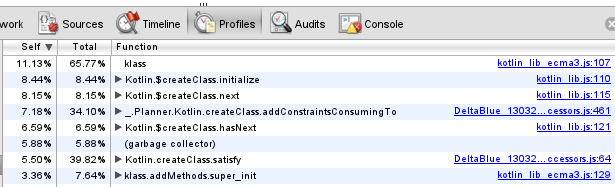
\includegraphics[width=0.7\textwidth]{img/deltablue_0_profile.png}
\caption{Результаты сбора профилировочной информации на тесте DeltaBlue}
\label{deltablue_0_prifile}
\end{figure}

На рисунке \ref{deltablue_0_prifile} приведены результаты профилирования теста DeltaBlue. Как видно, много времени тратится на конструирование объектов, причем существенную долю этого времени занимает работа инфраструктурного кода. Как можно видеть на рисунке \ref{deltablue_i}, экспериментально удалось подтвердить, что ускорить конструирование объектов в рамках существующей структуры возможно.

\newpage
Приведем простой пример демонстрирующий данную проблему (листинги \ref{constructor_problem_kt} и \ref{constructor_problem_js}):

\begin{code}
\begin{Kotlin}[caption=Пример с наследованием, label=constructor_problem_kt]
open class A(val name: String)

class B(name: String) : A(name)
\end{Kotlin}
\end{code}

\begin{code}
\begin{JavaScript}[caption=Результат компиляции примера с наследованием, label=constructor_problem_js]
(function () {
  'use strict';
  var classes = function () {
    var c0 = Kotlin.createClass({
      initialize: function (name) {
        this.name = name;
      }
    });
    return {c0: c0};
  }()
  , _ = {
    A: classes.c0,
    B: Kotlin.createClass(classes.c0, {
      initialize: function (name) {
        this.super_init(name);
      }
    })
  };
  Kotlin.defineModule('JS_TESTS', _);
}());
\end{JavaScript}
\end{code}

% \newpage
Первая проблема заключается в том, что при создании <<класса>> вызов функции инициализатора \path{initialize} оборачивается в библиотечную функцию \path{klass} (см. листинг \ref{klass_js}), вызов которой мы и наблюдаем в профилировщике, что создает дополнительные расходы при создании объектов -- в виде еще одного вызова функции. Данную проблему можно решить, избавившись от функции обертки и использованием пустого инициализатора в случае отсутствия своего инициализатора у создаваемого класса.

\begin{code}
\begin{JavaScript}[caption=Функция klass из стандартной библиотеки, label=klass_js]
function klass() {
    this.initializing = klass;
    if (this.initialize) {
        this.initialize.apply(this, arguments);
    }
}
\end{JavaScript}
\end{code}

Следующая проблема связана с вызовом конструктора наследуемого класса, который реализуется в виде вызова функции \path{super_init}, код которой приведен в листинге \ref{super_init_js}. Что вновь создает накладные расходы при создании экземпляров класса с предком отличным от \path{Any}.

\begin{code}
\begin{JavaScript}[caption=Функция super\_init из стандартной библиотеки, label=super_init_js]
function super_init () {
	this.initializing = this.initializing.superclass;
	this.initializing.prototype.initialize.apply(this, arguments);
}                
\end{JavaScript}
\end{code}

Для решения данной проблемы было решено заменить генерацию, в теле инициализатора, вызова функции \path{super_init} на <<прямой>> вызов конструктора суперкласса. Для приведенного ранее примера (листинг \ref{constructor_problem_kt}) такой код будет выглядеть следующим образом:

\begin{code}
\begin{JavaScript}[caption=Результат компиляции примера с наследованием(листинг \ref{constructor_problem_kt}) с прямым вызовом конструктора суперкласса, label=constructor_problem_js_fixed]
(function () {
  'use strict';
  var classes = function () {
    var c0 = Kotlin.createClass({
      initialize: function (name) {
        this.name = name;
      }
    });
    return {c0: c0};
  }()
  , _ = {
    A: classes.c0,
    B: Kotlin.createClass(classes.c0, {
      initialize: function (name) {
        A.call(this, name);
      }
    })
  };
  Kotlin.defineModule('JS_TESTS', _);
}());
\end{JavaScript}
\end{code}

Также была оптимизирована реализация функции \path{Kotlin.equals}, которая используется для сравнения объектов и, судя по результату профилировки, тоже вызывается достаточно часто. И было оптимизировано сравнение примитивных типов, которое осуществлялось через вызов функции \path{Kotlin.equals}, в то время как было бы достаточно и оптимальнее использовать оператор \path{===}.

Реализованные оптимизации позволили значительно улучшить результаты кода, скомпилированного с помощью компилятора Kotlin. На рисунке \ref{deltablue_f} можно видеть, что итоговые результаты очень близки к результатам компилятора Dart2js.


Кроме того, в результате исследования кода, полученного после компиляции теста DeltaBlue, были сделаны следующие выводы:
\begin{itemize}
\item Необходимо пересмотреть реализации контейнеров в стандартной библиотеке.
\item Необходимо, когда это возможно, на этапе компиляции заменять используемые контейнеры на <<родные>> для JavaScript аналоги.
\item Не использовать \path{Kotlin.equals} для проверки ссылочной эквивалентности объектов.
\end{itemize}

\begin{figure}[ht!]
\centering
\begin{minipage}[t]{\linewidth}
\includegraphics[width=0.8\textwidth]{images/deltablue_f.png}
\end{minipage}

\begin{minipage}[h]{\linewidth}
\centering
\begin{tabular}{|l|c|c|}
    \hline
    ~                       & Время (мкс) & Фактор \\ \hline
    Dart                    & 5321.81     & 1.0    \\ \hline
    Dart2JS(v8)             & 6900.66     & 1.30   \\ \hline
    JavaScript (v8)         & 5494.51     & 1.03   \\ \hline
    Kotlin2JS (v8)          & 1347000     & 253.10 \\ \hline
    Kotlin2JS OPT (v8)      & 8950.89     & 1.68   \\ \hline
    Dart2JS(mozjs17)        & 50550       & 9.50   \\ \hline
    JavaScript (mozjs17)    & 10837.83    & 2.04   \\ \hline
    Kotlin2JS (mozjs17)     & 563000.65   & 105.79  \\ \hline
    Kotlin2JS OPT (mozjs17) & 62750     & 11.79  \\ \hline
\end{tabular}
\end{minipage}
\caption{Итоговый результат на тесте DeltaBlue}
\label{deltablue_f}
\end{figure}

% \newpage
\section{Havlak}

Результаты, полученные на начальном этапе, без использования оптимизаций, на тест Havlak представленны на рисунке \ref{havlak_0}.

\begin{figure}[ht!]
% \centering
\begin{minipage}[t]{\linewidth}
\includegraphics[width=0.65\textwidth]{images/havlak_0.png}
\end{minipage}
~
\put(-173,175){\begin{minipage}[h]{\linewidth}
\begin{tabular}{|l|c|c|}
    \hline
    ~                    & Время (мс) & Фактор \\ \hline
    Dart                 & 654        & 1.0    \\ \hline
    Dart2JS(v8)          & 1685       & 2.58   \\ \hline
    JavaScript (v8)      & 2401       & 3.67   \\ \hline
    Kotlin2JS (v8)       & 103371     & 158.06 \\ \hline
    Dart2JS(mozjs17)     & 20637      & 31.56  \\ \hline
    JavaScript (mozjs17) & 2534       & 3.87   \\ \hline
    Kotlin2JS (mozjs17)  & 52893      & 80.88  \\ \hline
\end{tabular}
\end{minipage}}
\caption{Результаты теста Havlak без оптимизаций}
\label{havlak_0}
\end{figure}

На диаграмме видно, что снова быстрее всех код написанный на Dart и выполняющийся в DartVM. Следом идет, как ни странно, результат скомпилированный с помощью Dart2js. Это объясняется тем что в реализации на JavaScript \cite{HavlakBench:src} часто используемый фрагмент был реализован не очень оптимально, а именно то, что в качестве ключа ассоциативного массива используется объект(см. листинг \ref{example_BaseBlock}).

\begin{code}
\begin{JavaScript}[caption=Пример неоптимального использования ассоциативного массива на JavaScript, label=example_BaseBlock]
...
function BasicBlock(name)
{
  this.name = name;
  ...
}

BasicBlock.prototype.toString = function() {
  return "BB" + this.name;
}
...
function DFS(currentNode, nodes, number, last, current) {
...
  number[currentNode] = current;
...
}
\end{JavaScript}
\end{code}

Данное решение неоптимально, потому что при каждом обращение к такому массиву виртуальная машина вызывает у объекта метод toString, а в этом методе каждый раз осуществляется конкатенация двух строк, одна из которых получается преобразованием числа из поля \path{name} в строку. Эксперименты показали, что если для доступа к объектам ассоциативного массива использовать не объект а, например, поле \path{name}, как в листинге \ref{example_BaseBlock_fixed}, то тест будет выполнятся в два раза быстрее.

\begin{code}
\begin{JavaScript}[caption=Пример улучшения использования ассоциативного массива в тесте на JavaScript, label=example_BaseBlock_fixed]
...
function DFS(currentNode, nodes, number, last, current) {
...
  number[currentNode.name] = current;
...
}
\end{JavaScript}
\end{code}

\begin{figure}[ht!]
\centering
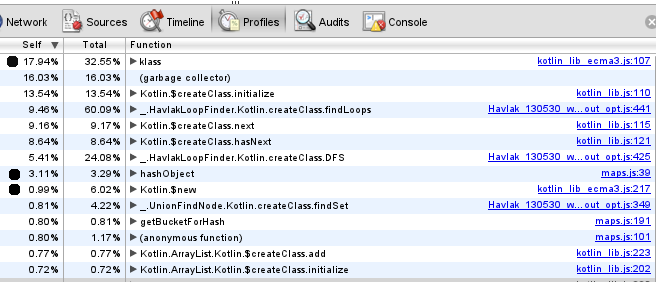
\includegraphics[width=0.8\textwidth]{img/havlak_0_profile.png}
\caption{Результаты профилирования на тесте Havlak}
\label{havlak_0_profile}
\end{figure}

На рисунке \ref{havlak_0_profile} представлены результаты профилирования кода, полученного компилятором Kotlin. Наибольший интерес для нас представляют функции из стандартной библиотеки. Это связанно с тем, что нашей главной целью является увеличение общей производительности, а не просто увеличение скорости выполнения конкретного теста. В результате изучения кода были отобраны функции, которые нуждаются в оптимизации. На рисунке, такие функции помечены точкой в начале строки. В отношении остальных функций было решено, что они достаточно оптимальны.

\begin{figure}[ht!]
% \centering
  \begin{subfigure}[b]{0.65\textwidth}
  \begin{minipage}[t]{\linewidth}
  \includegraphics[width=\textwidth]{images/havlak_i_v8.png}
  \end{minipage}
  ~
  \put(-10,211){\begin{minipage}[h]{\linewidth}
  \begin{tabular}{|l|c|}
      \hline
      ~                       & Время (мс)  \\ \hline
      Kotlin2JS(без изм.)     & 103371      \\ \hline
      +Inline акc. и пакеты   & 78110       \\ \hline
      +Kotlin.\$new -> new    & 5095       \\ \hline
      +оптмизация hashObject  & 3667        \\ \hline
      +PrimitiveHashMap       & 1641        \\ \hline
  \end{tabular}
  \end{minipage}}

  \caption{Результаты измерений на V8}
  \end{subfigure}

  \begin{subfigure}[b]{0.65\textwidth}
  % \centering
  \begin{minipage}[t]{\linewidth}
  \includegraphics[width=\textwidth]{images/havlak_i_mozjs17.png}
  \end{minipage}
  ~
  \put(-10,211){\begin{minipage}[h]{\linewidth}
  \begin{tabular}{|l|c|c|}
      \hline
      ~                       & Время (мс)  \\ \hline
      Kotlin2JS(без изм.)     & 103371      \\ \hline
      +Inline акc. и пакеты   & 69744       \\ \hline
      +Kotlin.\$new -> new    & 11989       \\ \hline
      +оптмизация hashObject  & 7406        \\ \hline
      +PrimitiveHashMap       & 5615        \\ \hline
  \end{tabular}
  \end{minipage}}
  \caption{Результаты измерений на mozjs17}
  \end{subfigure}
\\*``+'' означает что изменения накладываются на предыдущее
\caption{Оптимизация кода сгенерированного на тесте Havlak}
\label{havlak_i}
\end{figure}

\newpage
Как видно, больше всего времени программа проводит в коде конструктора -- функция \path{klass}, что еще раз свидетельствует о необходимости оптимизировать процесс конструирования объектов. Результаты применения этой оптимизации можно видеть на рисунке \ref{havlak_i}.

Следующая интересная для нас функция это \path{Kotlin.$new}. Данная функция использовалась для старой реализации наследования, но в текущей реализации она уже не нужна. Поэтому данная функция была удалена, в результате чего был получен большой прирост скорости, который можно наблюдать на рисунке \ref{havlak_i}.

В тесте Havlak очень активно используются ассоциативные массивы и от качества их реализации во многом зависит итоговый результат.
На рисунке с результатом профилирования (\ref{havlak_0_profile}) это можно наблюдать ввиде вызовов функций \path{hashObject} и \path{getBucketForHash}.

Функция \path{hashObject} используется в базовом классе для ассоциативных контейнеров \path{Hashtable} для получения хеша объекта. Оригинальная версия данной функции представлена в листинге \ref{hashObject_original}.

В JavaScript при реализации ассоциативных массивов обычно пользуется тем, что во время выполнения объектам языка (Object) можно добавлять и удалять свойства. Для работы с такими свойствами используется их строковое представление~\cite{EffJS}. Зная это, можно понять почему функция \path{hashObject} возвращает строку.

Данная реализация имеет два основных недостатка:
\begin{enumerate}
\item Нет отдельной обработки чисел, в результате чего каждое обращение к числу как объекту, во время проверки наличия у него методов \path{hashCode} и \path{toString}, приводит к его преобразованию в \path{Object}. Далее это число преобразуется в строку, не смотря на то, что такое преобразование будет осуществлено при обращении к свойству.
Кроме того, такое преобразование чисел в строку может лишить виртуальную машину возможности оптимизировать обращения к индексированным свойствам объекта.

\item Для объектов, которые явно не реализуют функцию \path{toString}, в соответствии со стандартом \cite{ES5}, мы всегда будем получать один и тот же результат -- <<[object Object]>>. Что приведет к тому, что все такие объекты будут попадать в одну группу.
\end{enumerate}

\begin{code}
\begin{JavaScript}[caption=Оригинальная версия функции hashObject, label=hashObject_original]
function hashObject(obj) {
    var hashCode;
    if (typeof obj == "string") {
        return obj;
    }
    else if (typeof obj.hashCode == FUNCTION) {
        // Check the hashCode method really has returned a string
        hashCode = obj.hashCode();
        return (typeof hashCode == "string") ? hashCode : hashObject(hashCode);
    }
    else if (typeof obj.toString == FUNCTION) {
        return obj.toString();
    }
    else {
        try {
            return String(obj);
        }
        catch (ex) {
            // For host objects (such as ActiveObjects in IE) that have no toString() method and throw an error when
            // passed to String()
            return Object.prototype.toString.call(obj);
        }
    }
}
\end{JavaScript}
\end{code}

Для исправления первого недостатка была добавлена соответствующая логика, которая возвращает входной аргумент, без преобразований, если он имеет числовой тип (\path{number}).

Для исправления второго недостатка была изменена логика работы функции для случая отсутствия у объекта реализации функции \path{hashCode}. В предлагаемой реализации в случае наличия специального поля \path{$hashCode} возвращается значение данного поля. Иначе, с помощью функции \path{nextHashCode} получается новый хеш-код, который сохраняется в специальное поле \path{$hashCode}, для последующего использования, и возвращается как результат функции.
Функция \path{nextHashCode} имеет простую реализацию и может быть легко изменена. Кончено же, в идеале, такая функция должна возвращать случайное значение, но эксперименты показали, что реализация такой функции, в плане производительности, обходится слишком дорого, даже при использовании стандартных функций \path{Number.random()} и \path{Date.now()}. Поэтому было решено оставить данную реализацию как самую быструю и простую.
Получившиеся результат приведен в листинге \ref{hashObject_new}.

\begin{code}
\begin{JavaScript}[caption=Новая версия функции hashObject, label=hashObject_new]
var HASH_CODE = 0;
function nextHashCode() {
    var hash = HASH_CODE;
    HASH_CODE = (HASH_CODE + 1) | 0;
    return hash;
}

function hashObject(obj) {
    if (obj == null)
        return obj;

    var objType = typeof obj;
    if (objType === "string" || objType === "number") {
        return obj;
    }
    else if (typeof obj.hashCode == FUNCTION) {
        // Check the hashCode method really has returned a string
        var hashCode = obj.hashCode();
        var hashCodeType = typeof hashCode;
        return (hashCodeType === "string" || hashCodeType === "number") ? hashCode : hashObject(hashCode);
    }
    
    if (obj.$hashCode === undefined) {
        obj.$hashCode = nextHashCode();
    }

    return obj.$hashCode;
}
\end{JavaScript}
\end{code}

В случае если в качестве ключа используется примитивный тип или закрытый класс, в котором не определена своя реализация функции \path{hashCode}, можно использовать более простую и быструю реализацию ассоциативного контейнера -- \path{PrimitiveHashMap}.
Для примитивных типов решение об использовании \path{PrimitiveHashMap} можно принимать на этапе компиляции. Для классов же такое решение не подходит, т.к. в определенных ситуациях это может нарушить <<бинарную>> совместимость. Поэтому было решено осуществлять выбор нужно контейнера во время выполнения. К сожалению, текущая структура классов (времени выполнения) не предоставляет информацию о закрытости типа из-за чего невозможно выполнить данную оптимизацию в полной мере.

%Можно сделать SmartHashMap

% \null
% \begin{LARGE}
% \begin{center}
% \textbf{Результаты}
% \end{center}
% \end{LARGE}

В результате проведенных оптимизаций удалось значительно улучшить результаты кода скомпилированного с помощью компилятора Kotlin. Итоговый результат приведен на рисунке \ref{havlak_f}.

\begin{figure}[ht!]
\centering
\begin{minipage}[t]{\linewidth}
\includegraphics[width=0.8\textwidth]{images/havlak_f.png}
\end{minipage}

\begin{minipage}[h]{\linewidth}
\centering
\begin{tabular}{|l|c|c|}
    \hline
    ~                       & Время (мкс) & Фактор \\ \hline
    Dart                    & 654        & 1.0    \\ \hline
    Dart2JS(v8)             & 1685       & 2.58   \\ \hline
    JavaScript (v8)         & 2401       & 3.67   \\ \hline
    Kotlin2JS (v8)          & 103371     & 158.06 \\ \hline
    Kotlin2JS OPT (v8)      & 1641       & 2.51   \\ \hline
    Dart2JS(mozjs17)        & 20637      & 31.56  \\ \hline
    JavaScript (mozjs17)    & 2534       & 3.87   \\ \hline
    Kotlin2JS (mozjs17)     & 52893      & 80.88  \\ \hline
    Kotlin2JS OPT (mozjs17) & 5615       & 8.59   \\ \hline
\end{tabular}
\end{minipage}
\caption{Итоговый результат на тесте Havlak}
\label{havlak_f}
\end{figure}

% \begin{itemize}
% \item Kotlin.\$new
% \item hashCode
% и контейнеры которые используют hashCode
% \item Заменить все контейнеры на родные для JS аналоги
% \end{itemize}